\emph{Narratology}, or narrative theory, is a literary science that has experienced considerable development over the last hundred years. The topic of narrative theory has been explored by literary theorists across Europe throughout the twentieth century. Consequently, a number of different typologies and proposals have emerged on how to view the topic of narrative and narrative mode, and how to conduct narrative analysis.

.\cite{kubicek-vypravec}

In this chapter I introduce some basic narratological concepts. Next, I show a selected typology to demonstrate its relevance to this thesis, ????? and focus on the application of narrative theory to creative writing.

\section{Foundations of Literary Theory and Narratology}

\subsection{Point of view}

Pojem \emph{point of view} lze do češtiny přeložit jako \emph{hledisko}. Hledisko je

TODO najít tu knihu s definicemi pojmů!

\subsection{Forms of narrative by person}

\emph{Person} is a linguistic category of verbs, on the basis of which the primary forms of narrative are distinguished.In addition to verbs, this form is also manifested in personal and possessive pronouns and some special conjunctions.
\paragraph{Ich-forma}

TODO kniha s definicemi

\paragraph{Du-forma}

\paragraph{Er-forma}

\subsection{System of narrative modes}

From a number of narrative typologies I decided to choose the system proposed by Czech linguist and literary theorist Lubomír Doležel. Doležel's system of narrative modes is captured in the tree diagram in the figure \ref{fig:schema-dolezel}.\cite{dolezel-narativni-zpusoby}

\begin{figure}[ht]
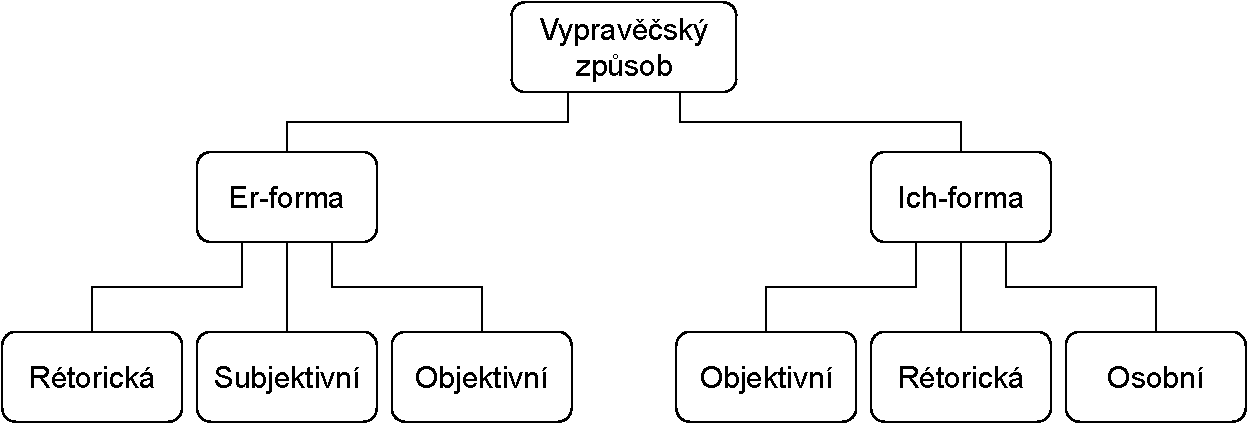
\includegraphics[width=1\textwidth]{data/dolezel-schema.pdf}
\caption{System of narrative modes by Doležel}
\label{fig:schema-dolezel}
\end{figure}



